\section{分块问题}
\label{sec:block-problem}

本节回答一个问题：把变量分成若干块、每次只动一块时，块应当怎样划分，块与块之间的哪些关系会妨碍这种做法。

\subsection{块的划分}
\label{sec:block-partition}

\paragraph{两个具体的问题}
先看最小二乘。设$\bm{A}\in\mathbb{R}^{N\times n}$，第$j$列记为$\bm{a}_j$，目标是
\[
 f(\bm{x})=\frac12\lVert\bm{A}\bm{x}-\bm{b}\rVert_2^2 .
\]
若其他系数不动，只改$x_j$，残差$\bm{r}=\bm{A}\bm{x}-\bm{b}$只沿$\bm{a}_j$变化。这时一列数据就够用，变量的一个分量自然成为一块。

再看矩阵分解。给定$\bm{Y}\in\mathbb{R}^{p\times q}$，寻找$\bm{U}\in\mathbb{R}^{p\times r}$、$\bm{V}\in\mathbb{R}^{q\times r}$，使$\bm{U}\bm{V}^\top$接近$\bm{Y}$，目标是
\[
 \lVert\bm{Y}-\bm{U}\bm{V}^\top\rVert_F^2 .
\]
这里最自然的一块不是单个元素，而是整个因子。固定$\bm{V}$后，目标关于$\bm{U}$是凸二次的，可以一次解出。

\paragraph{块与条件子问题}
两个例子的共同结构是：把坐标分成互不重叠的几组，每次只让一组变化。为了精确地谈论这件事，需要一套记号。

\begin{definition}[变量分块与条件子问题]
\label{def:block-partition}
把下标集$\{1,\ldots,n\}$划分为$B$个互不相交的非空子集$J_1,\ldots,J_B$，每个子集称为一个\term{变量块}（variable block）。对块$J$，记$\bm{x}_J\in\mathbb{R}^{\lvert J\rvert}$为$\bm{x}$在$J$上的分量，$\bm{U}_J\in\mathbb{R}^{n\times\lvert J\rvert}$为单位矩阵中由$J$对应的列组成的子矩阵，并记偏梯度
\begin{equation}
 \nabla_Jf(\bm{x})=\bm{U}_J^\top\nabla f(\bm{x}).
 \label{eq:block-partial-gradient}
\end{equation}
固定$\bm{x}$在其他块上的取值，把块$J$的取值换成$\bm{z}$，得到的函数
\begin{equation}
 \varphi_J(\bm{z};\bm{x})=f\bigl(\bm{x}+\bm{U}_J(\bm{z}-\bm{x}_J)\bigr)
 \label{eq:block-conditional}
\end{equation}
称为块$J$的\term{条件函数}（conditional function），在块$J$的允许集合上最小化它的问题称为\term{条件子问题}（conditional subproblem）。
\end{definition}

$\bm{U}_J\bm{h}$的作用是把长度为$\lvert J\rvert$的向量$\bm{h}$放回块$J$的位置，其余分量补零。单个坐标是块大小为$1$的特殊情形，下文的结论同时覆盖单坐标和多坐标的块。图~\ref{fig:block-columns-rows}(a)是这种划分的样子：绿色的一段正在变化，其余两段被固定。

\begin{BookInlineFigure}
  \centering
  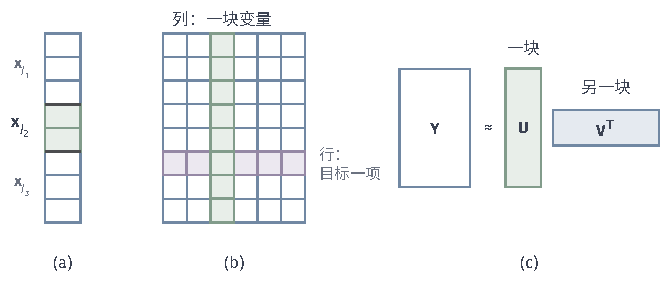
\includegraphics[width=112mm]{figures/05-optimization/04-block-optimization/tikz/block-columns-rows/figure.pdf}
  \caption{变量分块的三种形式。(a)向量$\bm{x}$分成三块，绿色的块$J_2$正在更新，其余块固定。(b)最小二乘的数据矩阵：选一列（绿）是选一块变量；选一行（紫）是选目标的一项，后者不属于本章的做法。(c)矩阵分解中，整个因子$\bm{U}$是一块。}
  \label{fig:block-columns-rows}
\end{BookInlineFigure}

图~\ref{fig:block-columns-rows}(b)还指出了一个容易混淆的区别。选列是在变量上做选择，读到的偏导数是准确的；选行是在目标的求和项上做选择，读到的方向只是全梯度的一个估计。两种选择回答不同的问题，也可以组合使用。选行带来的方向误差留到第~\ref{chap:stochastic-gradient-methods}章研究，本章的偏梯度都是精确的。

\paragraph{贯穿本章的例子}
全章反复使用同一个带交叉项的二元二次目标，起点固定为$(3,4)$：
\begin{equation}
 f(\bm{x})=x_1^2+x_1x_2+x_2^2,\qquad \bm{x}^{(0)}=(3,4).
 \label{eq:block-example}
\end{equation}
它的梯度和Hessian分别是
\[
 \nabla f(\bm{x})=\begin{bmatrix}2x_1+x_2\\x_1+2x_2\end{bmatrix},\qquad
 \bm{Q}=\begin{bmatrix}2&1\\1&2\end{bmatrix}.
\]
$\bm{Q}$的特征值是$1$和$3$，所以强凸常数$\mu=1$，光滑常数$L=3$，唯一的最优解是原点，$f^\star=0$。起点的目标值是
\[
 f(\bm{x}^{(0)})=9+12+16=37 .
\]

这个目标也是一个最小二乘问题。取
\[
 \bm{A}=\begin{bmatrix}1&1\\1&0\\0&1\end{bmatrix},\qquad \bm{b}=\bm{0},
\]
则$\bm{A}^\top\bm{A}=\bm{Q}$，并且$\tfrac12\lVert\bm{A}\bm{x}\rVert_2^2$展开后正是式~\eqref{eq:block-example}。对一般的$\bm{b}=\bm{A}\bm{x}^\star$，把变量平移成$\bm{x}-\bm{x}^\star$就回到$\bm{b}=\bm{0}$，这里取$\bm{0}$只是为了算起来干净。

\paragraph{一个坐标还是两个一起}
现在比较两种走法。按坐标更新时，把$x_2=4$固定，条件函数$z^2+4z+16$在$z=-2$取最小，走到$(-2,4)$；再固定$x_1=-2$，走到$(-2,1)$。

联合求解则把两个变量当成一块，解方程$\bm{Q}\bm{x}=\bm{0}$，一步到达原点。下表记录了目标值，图~\ref{fig:block-joint-vs-coordinate}是对应的路径。

\begin{BookInlineTable}
\centering
\begin{tabular}{lcc}
\toprule
做法 & 计算量 & 走完后的目标值\\
\midrule
更新$x_1$ & 一次除法 & $12$\\
再更新$x_2$ & 一次除法 & $3$\\
联合求解 & 解一个$2\times2$方程组 & $0$\\
\bottomrule
\end{tabular}
\end{BookInlineTable}

\begin{BookInlineFigure}
  \centering
  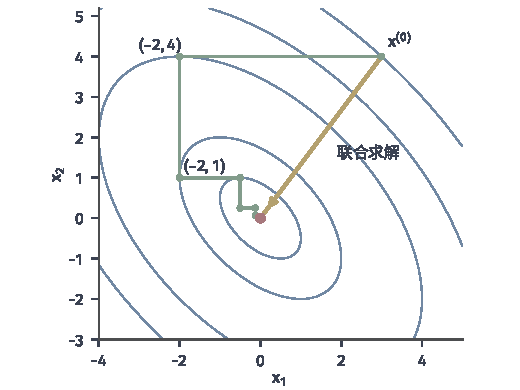
\includegraphics[width=88mm]{figures/05-optimization/04-block-optimization/matplotlib/block-joint-vs-coordinate/figure.pdf}
  \caption{式~\eqref{eq:block-example}上坐标更新与联合求解的比较。蓝色是等高线，绿色折线是依次精确更新$x_1$、$x_2$的前三轮，只能沿坐标轴方向走；黄色箭头是把两个变量当作一块、一步解出的路径；红点是最优解。}
  \label{fig:block-joint-vs-coordinate}
\end{BookInlineFigure}

块越大，每步的进展越大，但一步也越贵。这个交换关系在高维时才真正显出来。图~\ref{fig:block-size-cost}取$n=64$的链式二次目标，Hessian为三对角矩阵，主对角线上是$2.02$，次对角线上是$-1$，把相邻的$p$个变量分成一块，依次精确求解。

\begin{BookInlineFigure}
  \centering
  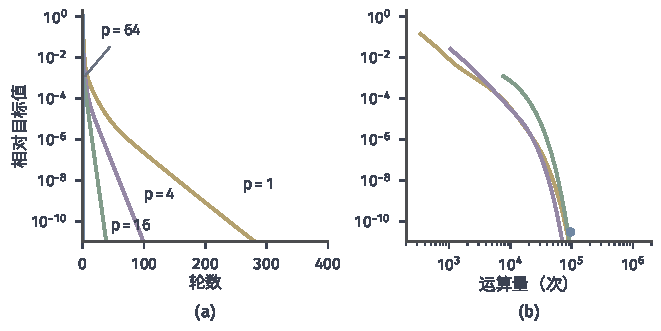
\includegraphics[width=112mm]{figures/05-optimization/04-block-optimization/matplotlib/block-size-cost/figure.pdf}
  \caption{块大小与计算量的交换。目标是$n=64$的链式二次函数，$p$个相邻变量为一块，循环精确更新。(a)相对目标值随轮数的变化，块越大轮数越少，$p=64$一轮即解出。(b)同一组数据按运算量画出，颜色与(a)相同，运算量按稠密块计：每块一次Cholesky分解计$p^3/3$，每次回代计$2p^2$，读取耦合项计$3p$，蓝点是$p=64$一次解出所用的运算量。}
  \label{fig:block-size-cost}
\end{BookInlineFigure}

以相对目标值降到$10^{-10}$为准，从(a)看，把块从$1$增大到$16$，所需轮数从$239$减到$34$，好像块越大越好。(b)把横轴换成运算量后，优势大半消失：四种块大小的总运算量都在$6\times10^4$到$10^5$之间，$p=4$反而最少。块大了一轮贵得多，轮数减少的好处被抵消了。选择块大小时，不能只看轮数。

\paragraph{决定块大小的三件事}
由此可以归纳出三个需要同时考虑的因素。第一是变量耦合：彼此强耦合的变量放进同一块，块内的联合求解才能消除这种耦合。第二是子问题的求解：块内要有闭式解、可复用的分解或便宜的迭代，否则分块省不下计算。

第三是数据读取：一块对应的数据最好能连续读取，并能借助残差之类的中间量增量维护，否则每次更新一块也要把数据读遍。

无论块怎样划分，评价进展时都看完整目标$f$，而不是当前块上条件函数的值。条件函数的最小值只说明这一块调到了最好，并不说明问题解决了。第~\ref{sec:block-exact}小节会用数字说明这个区别。

\subsection{块间耦合}
\label{sec:block-coupling}

上一小节的耦合只影响速度。有些耦合更严重，它让逐块更新根本走不动。本小节看两种情形，它们决定了后面每个算法都要检查的两个条件：可行性和可分性。

\paragraph{乘积可行域}
若可行集是各块集合的乘积
\begin{equation}
 \bm{C}=\bm{C}_{J_1}\times\cdots\times\bm{C}_{J_B},
 \label{eq:block-product-set}
\end{equation}
每一块只需留在自己的集合内，整个点就是可行的。各块的约束互不牵连，逐块更新可以自由进行。箱式约束$l_j\leq x_j\leq u_j$是最常见的例子，图~\ref{fig:block-feasible-coupling}(a)中沿任一坐标轴移动，只要不越过自己的边界，点就留在矩形内。

\paragraph{耦合约束}
情况在约束把几块绑在一起时完全不同。设$\bm{x}\in\mathbb{R}^n$满足$\sum_{j=1}^nx_j=1$，可行点$\bm{x}$的$x_j$改成$x_j+\delta$，分量之和就变成$1+\delta$。所以只要$\delta\neq0$就不可行，单坐标更新只能停在原地。

要在这个集合内移动，至少同时改两个坐标，让它们的变化互相抵消：
\[
 x_i\leftarrow x_i+\delta,\qquad x_j\leftarrow x_j-\delta .
\]
图~\ref{fig:block-feasible-coupling}(b)画出$n=3$的情形。红色的单坐标方向离开了三角形所在的平面，绿色的两坐标方向留在平面内。

\begin{BookInlineFigure}
  \centering
  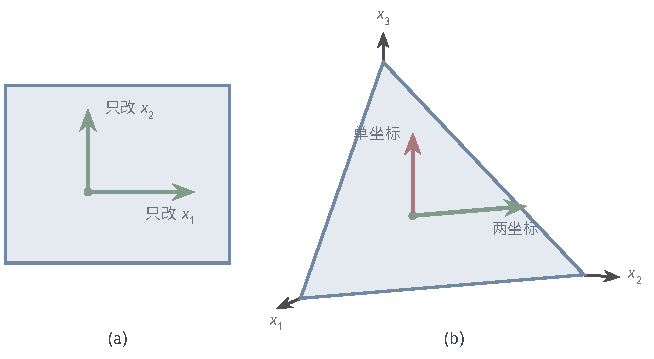
\includegraphics[width=108mm]{figures/05-optimization/04-block-optimization/tikz/block-feasible-coupling/figure.pdf}
  \caption{可行域与块的移动。(a)乘积可行域：矩形内的点沿任一坐标轴移动都可以留在可行域内。(b)$\sum_jx_j=1$的可行点（只画$x_j\geq0$的部分）：红色的单坐标移动离开平面，变得不可行；绿色的两坐标移动保持分量之和不变。}
  \label{fig:block-feasible-coupling}
\end{BookInlineFigure}

一般的耦合约束需要借助乘子把它们拆开，这部分内容放在第~\ref{chap:penalty-multiplier-methods}章。本章只讨论乘积可行域。

\paragraph{不可分的非光滑项}
另一种障碍来自目标本身。考虑凸函数
\begin{equation}
 F(u,v)=2\lvert u-v\rvert+\lvert u+v-2\rvert ,
 \label{eq:block-nonsmooth-example}
\end{equation}
它的最小值在$(1,1)$处取到，$F(1,1)=0$。把点放在原点，$F(0,0)=2$，看两个坐标方向能否改进。

固定$v=0$，条件函数是$F(u,0)=2\lvert u\rvert+\lvert u-2\rvert$，分段写出来就是
\[
 F(u,0)=\begin{cases}
 2-3u, & u<0,\\
 2+u, & 0\leq u\leq2,\\
 3u-2, & u>2.
 \end{cases}
\]
左边斜率为负，右边斜率为正，所以$u=0$是唯一的最小点。由$F$关于$u,v$的对称性，固定$u=0$时$v=0$也是唯一的最小点。

因此从原点出发，两个坐标都不肯动，算法永远停在目标值$2$处。可是沿对角线走却能下降：
\[
 F(s,s)=2\lvert s-1\rvert ,
\]
$s$从$0$增大到$1$时目标值从$2$降到$0$。图~\ref{fig:block-nonsmooth-stall}画出了这一情形。

\begin{BookInlineFigure}
  \centering
  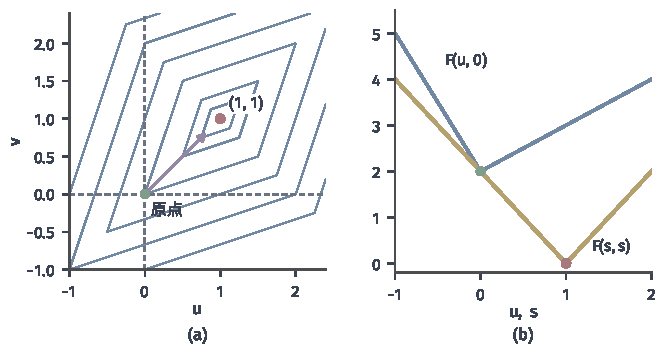
\includegraphics[width=112mm]{figures/05-optimization/04-block-optimization/matplotlib/block-nonsmooth-stall/figure.pdf}
  \caption{不可分非光滑项造成的坐标停滞。$F(u,v)=2\lvert u-v\rvert+\lvert u+v-2\rvert$。(a)蓝色是等高线，它们在折线上有尖角。绿点是原点，两条灰色虚线是过原点的坐标方向，紫色箭头指向最优解（红点）。(b)蓝线是坐标方向上的$F(u,0)$，在原点取最小；黄线是对角线方向上的$F(s,s)$，从原点继续下降。}
  \label{fig:block-nonsmooth-stall}
\end{BookInlineFigure}

原因在于原点恰好落在折线$u=v$上。原点附近$u+v-2<0$，于是
\[
 F(u,v)=2\lvert u-v\rvert+2-u-v .
\]
方向$(d_1,d_2)$要下降，必须满足$2\lvert d_1-d_2\rvert<d_1+d_2$，这些方向夹在$(3,1)$和$(1,3)$之间，是以对角线为中心的一个窄角，两个坐标方向都在窄角之外。

可以想象站在一条斜向的沟底，沿沟走是下坡，朝东西或南北走都会撞上沟壁。这个类比只对应“沿坐标方向不能下降”这一点：沟底是目标的尖角，光滑的目标没有这样的沟壁。如果$F$可微，两个偏导数都为零意味着梯度为零，这种事就不会发生。

这两种情形提醒我们，后面每个算法都要回答两个问题：只改一块时点还可行吗？非光滑项能按块拆开吗？第~\ref{sec:block-limits}小节还会回到这个反例，把“每块都不能改进”与“整体最优”的差别说清楚。
